\title{Computer Architecture - CS 301} % You may change the title if you want.

\author{Rishit Saiya - 180010027, Assignment - 13}

\date{\today}

\documentclass[12pt]{article}
\usepackage{fullpage}
\usepackage{enumitem}
\usepackage{amsmath,mathtools}
\usepackage{amssymb}
\usepackage[super]{nth}
\usepackage{textcomp}
\usepackage{hyperref}
\hypersetup{
    colorlinks=true,
    linkcolor=blue,
    filecolor=magenta,      
    urlcolor=cyan,
}
\begin{document}
\maketitle

%----------------------------------------------------------------

\section{}
\subsection{Port Mapped I/O}
Basically, in the Network Layer in the I/O stack. The Network Layer is primarily concerned with routing messages between different I/O devices. This layer also ensures that these messages reach their correct destinations. So, every device on the Motherboard exposes a set of I/O ports. \\

An I/O port in this context, is a software entity. It means that we have software interface as mentioned in the video lecture and is shown in Figure 1 also.

\begin{figure}
    \centering
    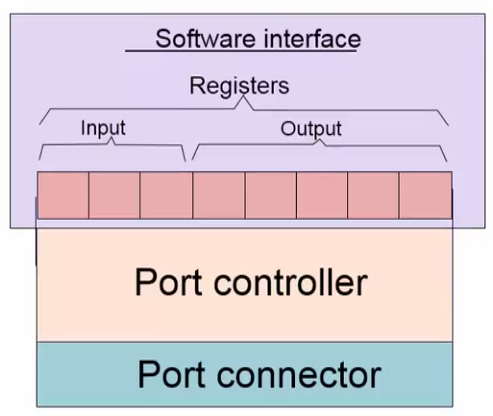
\includegraphics[width=12cm, height=10cm]{Assignment-13/port_add.png}
    \caption{Port Diagram}
\end{figure}

We have registers in the software interface from which we read and write. The Port Controller takes the data from the registers and performs proper formatting and Error checks (processing the Physical and Data Link Layer). A port connector is set of copper lead wires which help to get connected to external port. Each software I/O port is a wrapper on the actual hardware I/O port. \\

As mentioned in lecture, each I/O port exposes a set of 8-32 bit registers to software which essentially constitutes the address. A request contains an I/O port address. Software writes to the registers. The CPU/Processor sends it to the Northbridge Clip and then Northbridge Chip forwards it to the Southbridge chip. The Southbridge chip forwards it to the destination (I/O Device). Each chip maintains a routing table with Port Number and corresponding device. The response will trivially follow the reverse path. Similarly, to read data the processor reads the registers of the port controller. Example: Intel processors define 64K, 8 bit I/O ports. Each port has a 16 bit port number. \\

Some of the problems encountered with Port Mapped I/O are as follows:
\begin{itemize}
    \item Same device will have different port address across different motherboards as CPU allots port number when device connected.
    \item Since the data is sent instruction by instruction, this makes Block Data transfer slow.
    \item All the programs won't be portable on different CPUs or other processors.
    \item All the addresses of the I/O ports have to be explicitly known.
\end{itemize}

\subsection{Memory Mapped I/O}
In Memory Mapped I/O, we define a virtual layer between I/O ports and the software. However, software will not be actually aware of the address of I/O ports. The OS uses paging mechanism to map I/O ports to memory address. When we write to a memory address that is mapped to an I/O port, the TLB directs the request to I/O system for device. Similarly, for reading data, response travels back from I/O system. \\

Some of the problems encountered with Memory Mapped I/O are as follows:
\begin{itemize}
    \item All the addresses of the I/O ports have to be explicitly known.
    \item Programs will cease to work.
    \item Since the data is sent instruction by instruction, this makes Block Data transfer slow.
    \item The same device might have different port addresses across different motherboards, so in that case mapping would become extremely tedious.
\end{itemize}

Some of the advantages with Memory Mapped I/O are:
\begin{itemize}
    \item The same I/O program is now portable and can run on different machines.
    \item Easy to read/write large block of data using block load/store operations.
    \item Reading/Writing to I/O devices requires normal load/store instructions.
    \item The OS creates the mapping between the I/O ports the memory addresses.
\end{itemize}

%----------------------------------------------------------------

\section{}
Before jumping over to methods of Protocol Layer, it is important to understand the function of Protocol Layer in I/O Stack. \\

\textbf{Protocol Layer:} This layer defines the interaction between the host (processor) and I/O devices. The protocol layer consists of high level commands that are sent over the three lower layers. For this function, some of the methods are Polling, Interrupt and Direct Memory Access, which we will discussing below.

\subsection{Polling}
Polling is a method where an application running is functioned based on availability. It follows the following logic to function:
\begin{verbatim}
    Request = Preform Task (X);
    if (Processor(Busy)){
       Wait;
       Continue to Query until Processor(Free);
    }
    else{
       Send Contents for Task (X)
       Execute Task (X)
    }
\end{verbatim}
This method is known as Polling.

In the lecture video, this concept of Polling has been explained using Printer as a processor and Printing task as an example. It is assumed that the application running on the processor wants to print a page. It needs to first find if the printer is free before sending it the contents of the page. It keeps querying the printer for its status. If its status is busy, the program waits for some time, and queries again. Once the status is free, it sends the contents and Printing task is executed. This method is logically simple but rather inefficient due to constant traffic, power consumption and increased computation time. \\

\subsection{Interrupt}
In this, the host tells the processor to notify it if there is a change in its status. The Interrupts which can potentially be occurring in Polling are as follows:
\begin{itemize}
    \item The host tells the device to notify it if there is a change in its status.
    \item In this case, if the printer is busy, then the host lets the printer know that its interested in printing one more page.
    \item The host processes the interrupt and the application sends the printer job request.
    \item The printer sends it an interrupt, once it is free.
\end{itemize}
   

\subsection{Direct Memory Access}
As mentioned in the previous logic about sending contents for Task (X), if the processor is free. But in the process of sending contents, the processor needs to transfer several MBs of data back to memory while performing Task (X). If it transfers byte by byte, then processor's status would be busy for practically entire time. \\

So, in order to avoid such blockage, Direct Memory Access (DMA) Engine is designed for transferring data between main memory and I/O device. DMA is typically part of Northbridge Chip. The Engine has access to main memory, and to I/O devices. It can seamlessly transfer data between them. Once Task (X) is done, an interrupt is sent to the processor. The processor programs the DMA engine with the addresses in memory, size of data, and I/O address locations. \\

Similar analogy for Printer Task for DMA task has been explained in the lecture and it is trivial here to understand it since the logic has been mentioned above. This DMA engines function in following modes:

\begin{itemize}
    \item \textbf{Burst Mode:} \\
    Since the message to Device-2 cannot be sent since block is involved in Northbridge, Southbridge, Memory and Device-1. It locks the Front Side Bus (FSB) and the buses to the I/O device till the entire transaction is over. 
    \item \textbf{Cycle Stealing Mode:} \\
    In this mode, the main idea is to split the transactions. In this mode, the engine transfers the data in smaller chunks. In this way, the DMA traffic typically has a much lower priority than regular traffic and resulting in seamless operations.
 
\end{itemize}

%----------------------------------------------------------------
\end{document}